%\documentclass[10pt,a5paper]{memoir}
\documentclass[10pt,ebook]{memoir}

% usual packages loading:
\usepackage{fontspec}
\setmainfont{Calluna}
%\newfontface{\vectis}{EBH Alternates}
\usepackage{humanist}
\newfontface{\vectis}{Mezalia}
\newfontface{\priory}{Priory}
\newfontface{\inglesh}{Calluna Sans}
\usepackage[autocompile]{gregoriotex} % for gregorio score inclusion
\usepackage{multicol}
\usepackage{graphicx} % support the \includegraphics command and options
\usepackage[pass-fonts=true,program=/home/veronica/bin/lilypond]{lyluatex}
\usepackage{lettrine}
\usepackage[savepos]{zref}
\usepackage{multicol}
\setlength{\trimtop}{0pt}
\setlength{\trimedge}{0pt}
\settypeblocksize{173mm}{110mm}{*} % Was 101mm in a5
\setulmargins{*}{*}{1.4}
\setlrmargins{*}{*}{1.2}
\setheadfoot{\onelineskip}{2\onelineskip}
\setheaderspaces{*}{.8\onelineskip}{*}
\checkandfixthelayout

\tolerance=1000
\pretolerance=800

\grechangestyle{translation}{\itshape \fontsize{10}{11}\selectfont}
\newcommand\translationfont[1]{{\itshape \fontsize{10}{11}\selectfont #1}}

\renewcommand{\LettrineFontHook}{\fontspec{Priory.ttf}}

\grechangestyle{initial}{\priory \fontsize{30}{30}\selectfont}
\grechangestyle{annotation}{\tiny}

\grechangestaffsize{16}

\makepagestyle{myheadings}
%\makeevenfoot{myheadings}{}{\small A New Book of Old Hymns Fifth Edition 2025}{} % page numbers at the outside
%\makeoddfoot{myheadings}{}{\small A New Book of Old Hymns Fifth Edition 2025}{}
\makeoddfoot{myheadings}{}{}{} 
\makeevenfoot{myheadings}{}{}{} 
\makeevenhead{myheadings}{\thepage}{\textsc{\leftmark}}{} % small caps
\makeoddhead{myheadings}{}{\textsc{\rightmark}}{\thepage}

\createmark{section}{both}{nonumber}{}{}

\newcommand\invisiblesection[1]{%
  \refstepcounter{section}%
  \addcontentsline{toc}{section}{#1}%
  \sectionmark{#1}
  \markboth{#1}{#1}}


\newcommand\hymntitle[1]{\subsection{#1}\index{#1}}
\setsubsecheadstyle{\centering\hminfamily\LARGE}
%\setbeforesecskip{-\onelineskip}
%\setaftersecskip{\onelineskip}

\newcommand\mysource[1]{\begingroup \raggedleft \footnotesize #1 \par \endgroup}

\makeindex

\newbox\linkbox
\newbox\wordbox
%\newdimen\boxwid

\def\lyrlink{%
  % Bogen erstellen: Put the smilie in the box:
  \setbox\linkbox=\hbox{$\smile$}%
  % In Box der Breite eines Wortzwischenraums einsetzen:
  % Make the box one space wide:
  \setbox\linkbox=\hbox to\the\fontdimen2\the\font{%
    \hss
    % Unter die Grundlinie druecken:
    % Lower the box under the word:
    \lower\ht\linkbox\hbox{%
      % Zusaetzlicher vertikaler Abstand zur Wortunterseite:
      % lower the smile a little bit more:
      \lower1pt\hbox{%
	\relax
	  \hbox{$\smile$}%
	}}%
    \hss}%
  % Keine zusaetzliche Tiefe fuer Bogen anrechnen:
  % Make the depth of the box zero:
  \dp\linkbox=0pt
  % Bogen setzen:
  \box\linkbox}

\def\intralink#1{%
  \setbox\linkbox=\hbox{$\smile$}%
  \setbox\wordbox=\hbox{#1}%
  \setbox\linkbox=\hbox to\wd\wordbox{%
    \hss
    % Unter die Grundlinie druecken:
    % Lower the box under the word:
    \lower\ht\linkbox\hbox{%
      % Zusaetzlicher vertikaler Abstand zur Wortunterseite:
      % lower the smile a little bit more:
      \lower1pt\hbox{%
	\relax
	  \hbox{$\smile$}%
	}}%
    \hss}%
  % Keine zusaetzliche Tiefe fuer Bogen anrechnen:
  % Make the depth of the box zero:
  \dp\linkbox=0pt
%  \let\boxwid=\the\wd\wordbox
%  \lower\ht\linkbox%
  \box\wordbox \llap{\box\linkbox}}

\newlength{\englishwidth}
\newlength{\latinwidth}
\newlength{\interwidth}
\newlength{\preverseskip}
\setlength{\englishwidth}{0.5\textwidth}
\setlength{\latinwidth}{0.48\textwidth}
\setlength{\interwidth}{10pt}
\setlength{\preverseskip}{10pt}
\newcounter{VerseNumber}

\newcommand\startverse[1]{\vskip\preverseskip\noindent\begin{minipage}[t]{\latinwidth}%
	\setcounter{VerseNumber}{#1}%
\hskip-3pt{#1 .}}
\newcommand\divverse{\end{minipage}%
	\hskip\interwidth%
\begin{minipage}[t]{\englishwidth}\itshape%
	\hskip-3pt{\theVerseNumber .} }
\newcommand\finishverse{\end{minipage}}

\newcommand\invoc[2]{\begin{minipage}[t]{0.5\textwidth}#1\end{minipage}\begin{minipage}[t]{0.5\textwidth}\textit{#2}\end{minipage}}

\setlength{\parindent}{0pt}

%% For the Litany:
\makeatletter  
\newcounter{score}
\newcounter{tabstop}[score]
\newcommand{\grealign}{%
	\@bsphack%
	\ifgre@boxing\else%
		\kern\gre@dimen@begindifference%
		\stepcounter{tabstop}%
		\expandafter\zsavepos{stop-\thescore-\thetabstop}%
		\kern-\gre@dimen@begindifference%
	\fi%
	\@esphack%
}

\newcommand{\setstops}{%
  \gdef\nstabbing@stops{%
    \hspace*{-\evensidemargin}\hspace{-1in}%
    \hspace*{\zposx{stop-\thescore-1} sp}\=%
  }%
  \count@=\@ne
  \loop\ifnum\count@<\value{tabstop}%
    \begingroup\edef\x{\endgroup
      \noexpand\g@addto@macro\noexpand\nstabbing@stops{%
        \noexpand\hspace{-\noexpand\zposx{stop-\thescore-\the\count@} sp}%
        \noexpand\hspace{\noexpand\zposx{stop-\thescore-\the\numexpr\count@+1} sp}\noexpand\=%
      }%
    }\x
    \advance\count@\@ne
  \repeat
  \nstabbing@stops\kill
}
\makeatother

\newenvironment{nstabbing}
  {\setlength{\topsep}{0pt}%
   \setlength{\partopsep}{0pt}%
   \tabbing%
   \setstops}
  {\endtabbing\stepcounter{score}}



\begin{document}
\pagenumbering{roman}
\pagestyle{empty}

\ 

\vfill

\begin{center}

	{\fontsize{32}{48} \hminfamily A New Book}

\quad


	{\fontsize{32}{48} \texthmin{of Old Hymns}}

\quad

\bigskip

	{\texthmin{ \LARGE in Latin and English}}

\quad


\bigskip

plainchant, polyphony,

\quad

sequences, a litany,

\quad


rounds, antiphons, carols

\quad


for all the seasons of the Church's year,

\quad


plus Ordinaries of the Mass,

\quad


Benediction

\quad


and some English hymns.

\vfill
\vfill

Fifth Edition

\end{center}

\vfill

\eject

\ 

\vfill

First Edition July 2004

Second Edition January 2006

Third Edition October 2007

Fourth Edition September 2014

Fifth Edition June 2025

Relevant recordings and resources at: newbookoldhymns.brandt.id.au


\bigskip

\begin{center}

New Book of Old Hymns © 2025 by Veronica Brandt \\
	is licensed under CC BY 4.0. \\
	To view a copy of this license, visit\\
	https://creativecommons.org/licenses/by/4.0/

	Published by Veronica Brandt www.brandt.id.au

ISBN: 978-1-312-60556-5

Imprint: Lulu.com

\end{center}

\eject

\tableofcontents*

\newpage


\ 

\vfill

\begin{center}
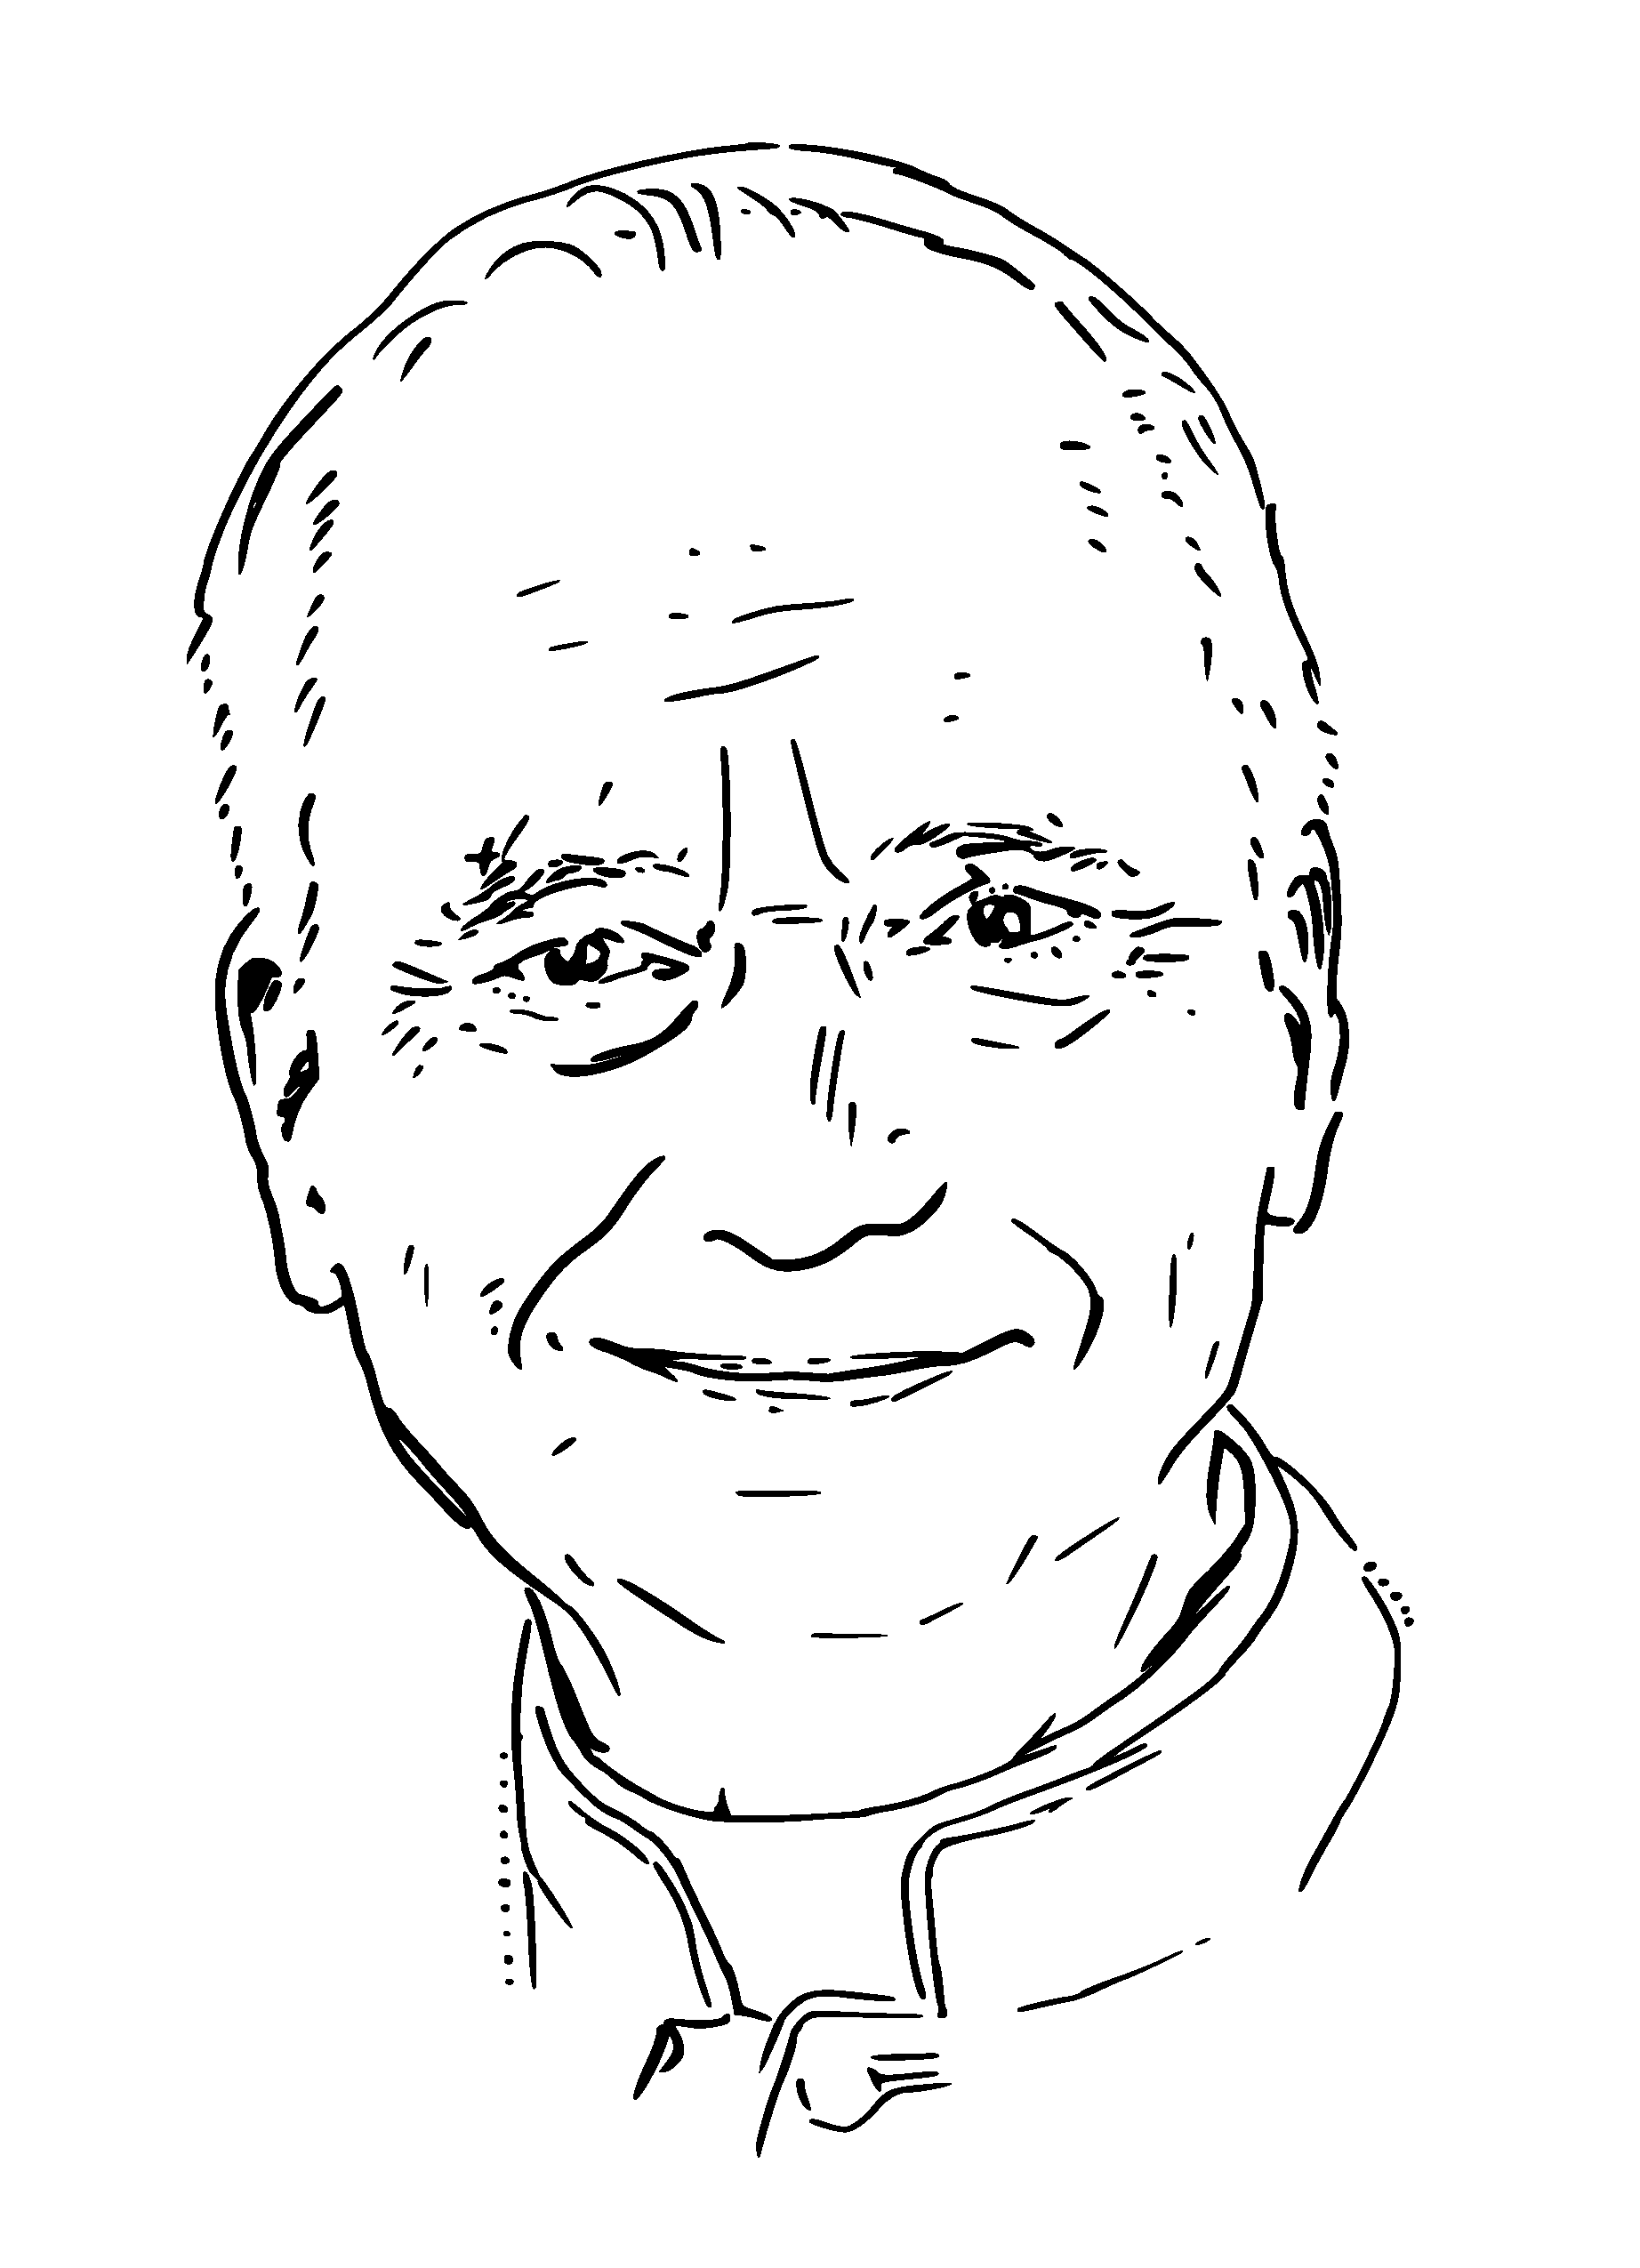
\includegraphics[width=5cm]{images/pope-leo-official}
\end{center}

\hymntitle{Oremus pro Pontifice nostro}
\index{Let us pray for our Pope}

\gregorioscore{gabc/va--oremus_pro_pontifice--solesmes}

\eject


\invisiblesection{Advent}

\setcounter{page}{1}
\pagenumbering{arabic}
\pagestyle{myheadings}

\hymntitle{Conditor alme Siderum}
\index{Creator of the starry skies}

\gregorioscore{gabc/hy--conditor_alme_siderum-v1--solesme}

\input conditor

\newpage

\hymntitle{Veni O Sapientia}
\index{O Come, O Come Emmanuel}

\input veniosapientia


\hymntitle{Rorate Caeli}
\index{Drop Down Dew}

\gregorioscore{gabc/va--rorate_caeli--solesmes.1}

\bigskip

\gregorioscore{gabc/va--rorate_caeli--solesmes.2}


\gregorioscore{gabc/va--rorate_caeli--solesmes.1}


\gregorioscore{gabc/va--rorate_caeli--solesmes.3}


\gregorioscore{gabc/va--rorate_caeli--solesmes.4}


\gregorioscore{gabc/va--rorate_caeli--solesmes.5}

\newpage


\invisiblesection{Christmas}

\hymntitle{Gaudete, gaudete}
\index{Rejoice, rejoice}

\input gaudete

\newpage

\hymntitle{Adeste, fideles}
\index{O Come, all ye Faithful}

\input adeste

\newpage

\hymntitle{Puer Natus in Bethlehem}
\index{A Boy is Born in Bethlehem}

\gregorioscore{gabc/hy--puer_natus_in_bethlehem--solesmes}

\input puernatus

\newpage


\invisiblesection{Holy Name}

\hymntitle{Jesu Dulcis Memoria}
\index{Jesus, the very thought of Thee}

\gregorioscore{gabc/hy--jesu_dulcis_memoria--solesmes}

\input jesu-dulcis

\begin{center}

\includegraphics[width=2cm]{images/ihs}
\end{center}

\newpage

\hymntitle{Non nobis, Domine}
\index{Not unto us, O Lord}

\input non-nobis

\hymntitle{Laudate Nomen Domini}
\index{Praise the Name of the Lord}

\input laudate

\invisiblesection{Epiphany}

\newpage


\invisiblesection{Candlemas}

\hymntitle{Lumen ad Revelationem Gentium}
\index{A Light to the Revelation of the Gentiles}

\input lumen.tex


\eject


\invisiblesection{Lent}

\grechangestyle{initial}{\priory \fontsize{28}{28}\selectfont}

\hymntitle{Attende Domine}

\input attende

\grechangestyle{initial}{\priory \fontsize{30}{30}\selectfont}
\newpage


\hymntitle{Parce Domine}


\input parce

\newpage


\invisiblesection{Passiontide}

%Gloria Laus
\hymntitle{Gloria Laus}
\index{All glory, laud and honour}

\gregorioscore{gabc/hy--gloria_laus--solesmes.1}

\gresetinitiallines{0}

\gregorioscore{gabc/hy--gloria_laus--solesmes.2}


\gregorioscore{gabc/hy--gloria_laus--solesmes.3}


\gregorioscore{gabc/hy--gloria_laus--solesmes.4}


\gregorioscore{gabc/hy--gloria_laus--solesmes.5}


\gregorioscore{gabc/hy--gloria_laus--solesmes.6}

\gresetinitiallines{1}

\bigskip

\mysource{St. Theodulf of Orleans, d.~821\\
Translated by J.~M.~Neale, 1818--66}

\newpage


\hymntitle{Vexilla Regis}
\index{Abroad the Regal Banners Fly}

\gregorioscore{gabc/hy--vexilla_regis_prodeunt--solesmes.1verse}

\input vexilla


\hymntitle{O Sacred Head sore wounded}

\input osacredhead

\newpage

\hymntitle{Ubi Caritas}
\index{Where there is Charity}

\gregorioscore{gabc/an--ubi_caritas--vatican}

\bigskip

\mysource{10th century\\
Some books give: Ubi caritas est vera – Where charity is true.}

\bigskip


\begin{center}

	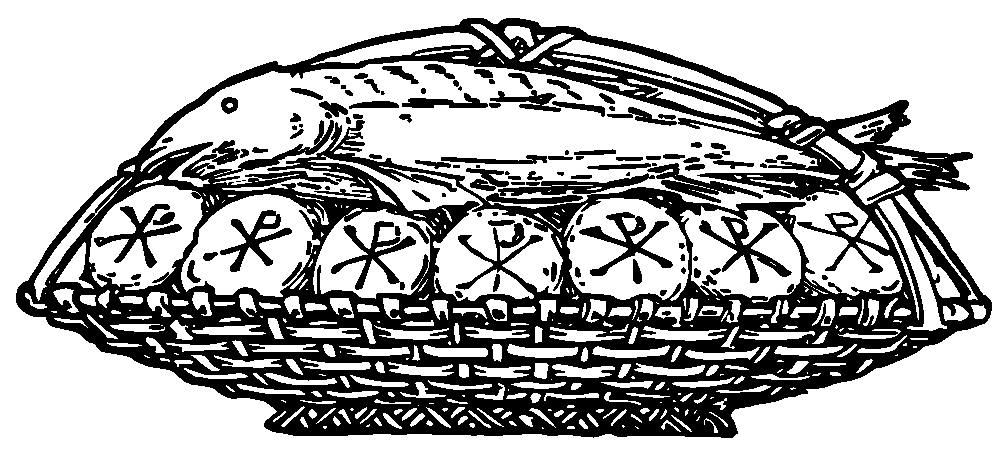
\includegraphics[width=5cm]{images/fishbread}

\end{center}


\newpage

\hymntitle{Pange Lingua}
\index{Sing, my tongue, the Saviour's glory}

\input pange

\newpage

\hymntitle{Stabat Mater dolorosa}
\index{By the Cross her station keeping}

\input stabat

\newpage

\hymntitle{Crux fidelis}
\index{Faithful Cross}
\index{Sing, my tongue, the glorious battle}
\index{Pange Lingua \ldots\ Lauream}

\input crux

\newpage

\invisiblesection{Easter}

\hymntitle{Haec dies}
\index{This is the day that the Lord hath made}

\gregorioscore{gabc/an--haec_dies--solesmes_1961.1}

\bigskip

\hymntitle{Jubilate Deo}

\input jubilate

\newpage

\hymntitle{O filii et filiae}
\index{O sons and daughters}

\input ofilii

\hymntitle{Alleluia}

This alleluia comes from Lauds of Easter Sunday.

\gregorioscore{gabc/co--alleluia--simplex}

\newpage

\hymntitle{Victimae paschali laudes}

\gregorioscore{gabc/se--victimae_paschali--solesmes.1}

\bigskip

\emph{Alternate translation:}

\index{Bring, all ye dear-bought nations}
\noindent\begin{minipage}[t]{0.5\textwidth}
\hskip-3pt 1. Bring, all ye dear-bought nations,\\
	\phantom{tab} bring\\
Your richest praises to your King,\\
	\phantom{tab} Alleluia, alleluia.\\
That spotless Lamb, who more than\\
	\phantom{tab} due,\\
Paid for His sheep, and those sheep\\
	\phantom{tab} you:\\
	\phantom{tab} Alleluia, alleluia,\\
	\phantom{tab} Alleluia, alleluia, alleluia.

	~

\hskip-3pt 2. That guiltless Son, who bought\\
	\phantom{tab} your peace,\\
And made His Father's anger cease,\\
	\phantom{tab} Alleluia, alleluia.\\
Then, Life and Death together\\
	\phantom{tab} fought,\\
Each to a strange extreme was\\
	\phantom{tab} brought:
\end{minipage}
\hskip6pt
\begin{minipage}[t]{0.5\textwidth}
\hskip-3pt 3. Life died, but soon revived again,\\
And even death by it was slain,\\
	\phantom{tab} Alleluia, alleluia.\\
Say, happy Magdalen, oh say,\\
What didst thou see there by the way?:

~

\hskip-3pt 4. ``I saw the tomb of my dear Lord,\\
I saw Himself and Him adored;\\
	\phantom{tab} Alleluia, alleluia.\\
I saw the napkin and the sheet,\\
That bound His hands and wrapped\\
	\phantom{tab} His feet:''

	~

\hskip-3pt 5. We, Lord, with faithful hearts and\\
	\phantom{tab} voice,\\
On this Thy rising day rejoice;\\
	\phantom{tab} Alleluia, alleluia.\\
O Thou, whose power o'ercame the\\
	\phantom{tab} grave,\\
By grace and love us sinners save:
\end{minipage}

\bigskip

\mysource{11th century\\
Translated by W.~K.~Blount, d.~1717}

\bigskip


\begin{center}
	
\includegraphics[width=3cm]{images/lamb}
\end{center}

\newpage

\hymntitle{Salve festa dies}
\index{Hail festal day}

\grechangestaffsize{15}

\gregorioscore{gabc/hy--salve_festa_dies--solesmes_1957.1}

\mysource{Venantius Fortunatus, 530--609}

\grechangestaffsize{16}
\newpage

\invisiblesection{Pentecost}

\hymntitle{Veni Sancte Spiritus}
\index{Holy Spirit, lord of light}

\gregorioscore{gabc/se--veni_sancte_spiritus_et_emitte--vatican}

\bigskip

\mysource{Ascribed to Stephen Langton, 12th century\\
Translated by Fr.~Edward Caswall, 1814--78}

\bigskip

\begin{center}
	
\includegraphics[width=8cm]{images/holyghost}
\end{center}

\newpage

\hymntitle{Veni Creator Spiritus}
\index{Come Holy Ghost}

\input venicreator

\newpage

\invisiblesection{Trinity}

\hymntitle{Firmly I believe}

\input firmly

\newpage


\invisiblesection{Corpus Christi}

\hymntitle{Adoro te devote}
\index{Godhead herein hiding}

\input adorote

\hymntitle{Anima Christi}
\index{Soul of my Saviour}

\input anima

\newpage

\hymntitle{Sacris solemniis}
\index{To the sacred feast}

\input sacris

\hymntitle{Sweet Sacrament divine}

\input sweet

\newpage

\hymntitle{Ave verum}
\index{Hail to Thee, True Body}

\gregorioscore{gabc/va--ave_verum--solesmes.1}

\mysource{Ascribed to Pope Innocent VI, 1362\\
Translation from the Roman Missal 1914\\
Tentatively ascribed to Fr.~E.~Caswall}

\newpage

\invisiblesection{Sacred Heart}

\hymntitle{To Jesus' Heart}

\input tojesus

\hymntitle{Cor Jesu Sacratissimum}
\index{Most Sacred Heart}

\gregorioscore{gabc/va--cor_jesu--solesmes.1}

\hymntitle{Glory be to Jesus}

\input glorybe

\newpage

\invisiblesection{Christ the King}

\hymntitle{Christus vincit}
\index{Christ conquers}

\input christus

\newpage

\invisiblesection{All Saints}

\hymntitle{Iste Confessor}
\index{This is the day whereon the Lord's true witness}

\input iste

\hymntitle{For all the Saints}

\input forall

\newpage

\hymntitle{Corda pia}

\gregorioscore{gabc/hy--corda_pia}

\input cordapia

\begin{center}
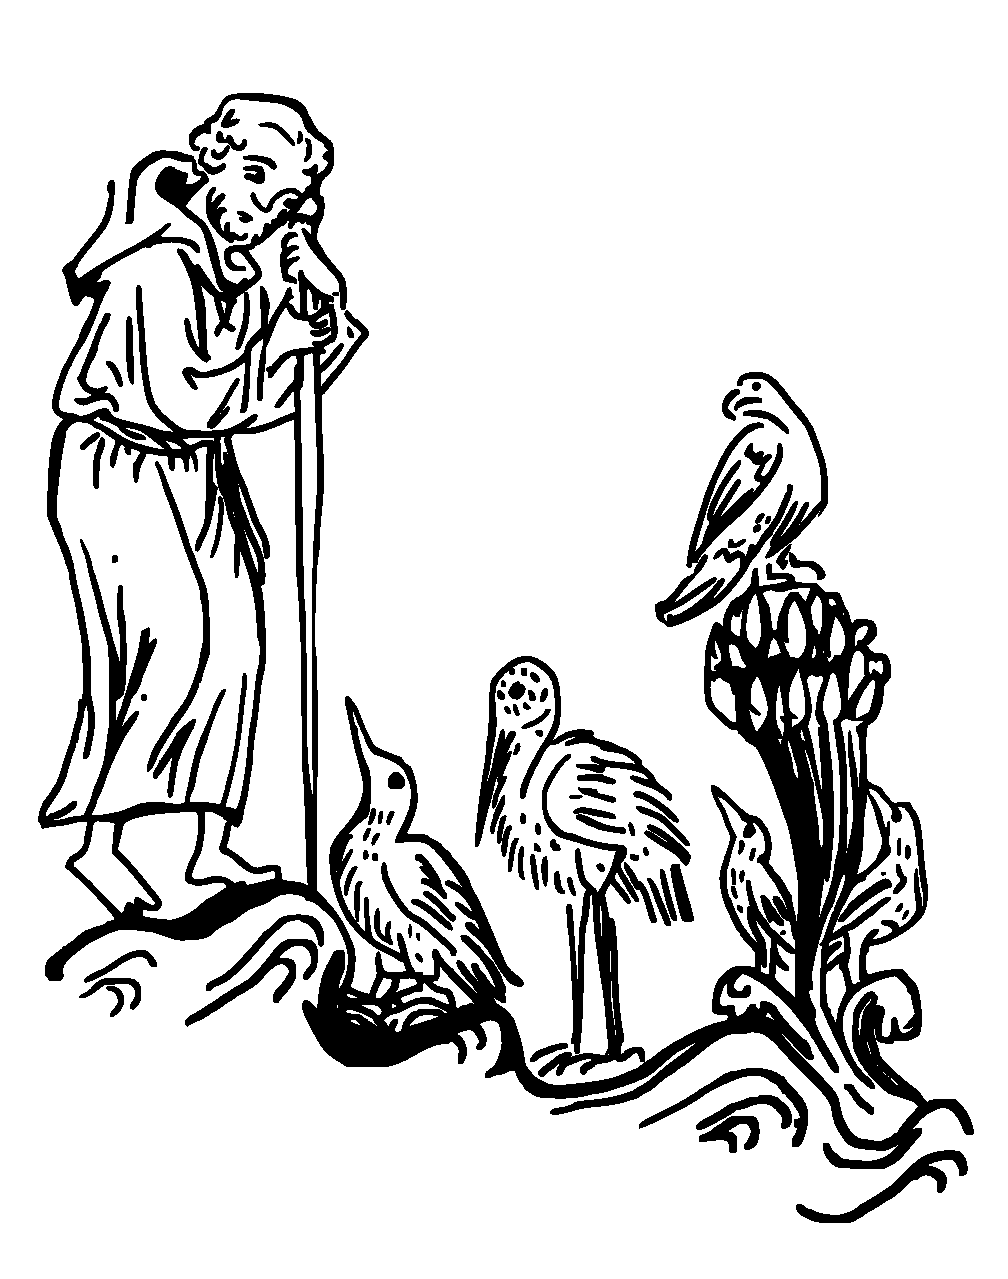
\includegraphics[width=6cm]{images/stfrancis}
\end{center}


\newpage

\invisiblesection{All Souls}

\hymntitle{Dies Irae}
\index{Day of Wrath}

\gregorioscore{gabc/se--dies_irae--vatican}

\emph{ the Saints' sweet rest.}

\mysource{Thomas of Celano, 13th century\\
Translated by Fr. J. Aylward, 1813--72\\
and William F. Wingfield, 1813--74}

\newpage

\hymntitle{Requiem Aeternam}
\index{Eternal Rest}

\gregorioscore{gabc/in--requiem--simplex}

\begin{center}

\includegraphics[width=4.8cm]{images/pall}
\end{center}


\newpage


\invisiblesection{Marian}

\hymntitle{Ave Maria}
\index{Hail Mary}

\gregorioscore{gabc/va--ave_maria_(salutatio_angelica)--solesmes_1961.1}

\bigskip

\emph{Alternate round setting:}

\lilypondfile{ly/ave-maria}

\bigskip

\emph{Another one from France:}

\lilypondfile{ly/ave-maria-ii}

\newpage

\hymntitle{Sub tuum praesidium}
\index{Under thy patronage}

\gregorioscore{gabc/an--sub_tuum_praesidium--solesmes_1934}

\hymntitle{Laudemus Virginem}

\begin{center}

\lilypondfile{ly/laudemus}

\end{center}

\mysource{Llibre Vermell de Monserrat}

\newpage

\hymntitle{Marian antiphons}

The marian antiphons are customarily sung after each hour of
the Divine Office according to the time of year. Alma Redemptoris
Mater is sung from the beginning of Advent through to Candlemas
(2nd February). Ave Regina Cælorum is sung from Candlemas
through Lent till Wednesday of Holy Week. No antiphons are
sung for the Sacred Triduum. Easter Sunday brings the Regina
Cæli which is also sung in place of the Angelus. After the Friday
after Pentecost the Salve Regina is sung.

\bigskip

\noindent\textbf{\large Alma Redemptoris Mater}
\index{Alma Redemptoris Mater}
\index{Beloved Mother of the Redeemer}

\gregorioscore{gabc/an--alma_redemptoris_(simple_tone)--solesmes_1961.1}

\mysource{Ascribed to Hermann of Reichenau, 1013--54}

\eject

\noindent\textbf{\large Ave Regina Caelorum}
\index{Ave Regina Caelorum}
\index{Hail Queen of Heavens}

\gregorioscore{gabc/an--ave_regina_caelorum--solesmes}

\bigskip

\noindent\textbf{\large Regina Caeli}
\index{Regina Caeli}
\index{O Queen of Heaven, rejoice!}

\gregorioscore{gabc/an--regina_caeli_laetare--solesmes}

\newpage

\noindent\textbf{\large Salve Regina}
\index{Salve Regina}
\index{Hail Holy Queen}

\gregorioscore{gabc/an--salve_regina_(simplex)--solesmes}

\newpage

\hymntitle{Stella splendens}

\input stella


\newpage

\hymntitle{Litany of Loreto}
\index{Litaniae Beatae Mariae Virginis}

\input litany

\begin{center}

\includegraphics[width=4cm]{images/rose}
\end{center}


\newpage

\hymntitle{Ave maris stella}
\index{Ave star@Ave, star of ocean}

\input avemaris

\newpage

\hymntitle{Virgo Dei Genitrix}
\index{Virgin Mother of God}

\input virgodei

\bigskip

\begin{center}
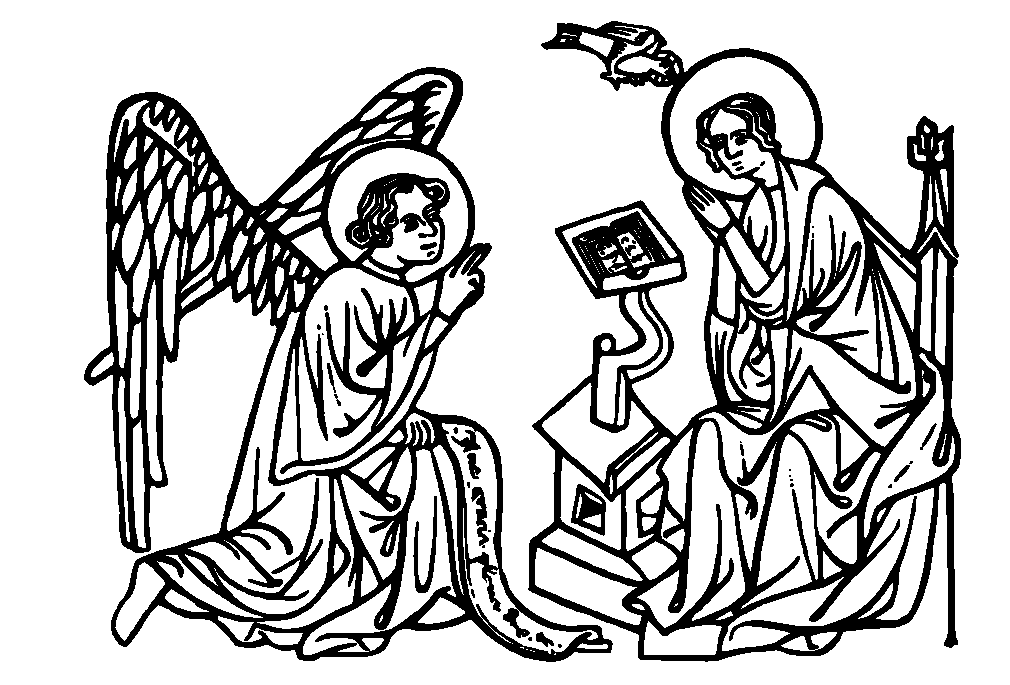
\includegraphics[width=7cm]{images/annun}
\end{center}

\newpage

\invisiblesection{For Peace}

\bigskip

\hymntitle{Dona nobis pacem}
\index{Grant us peace}

\input dona-nobis

\newpage

\hymntitle{Da Pacem Domine}
%\index{Grant peace, O Lord}

\gregorioscore{gabc/an--da_pacem_domine--solesmes}

\bigskip

\emph{Alternate round setting:}

\lilypondfile{ly/dapacem}

\bigskip


\emph{* The second and fourth parts comes in on ‘d’ and are sung a fourth below,
rather like Non nobis Domine p.~10.}

\bigskip


\mysource{Melchior Franck, 1580--1639}

\begin{center}

\includegraphics[width=3cm]{images/lily}
\end{center}


\newpage

\invisiblesection{Thanksgiving}

\hymntitle{Now thank we all our God}

\bigskip

\hskip3cm\begin{minipage}{7cm}
\lettrine{N}{ow} thank we all our God,\\
With heart and mind and voices,\\
Who wondrous things hath done,\\
In whom this world rejoices;\\
Who from our mother's arms\\
Hath blessed us on our way\\
With countless gifts of love,\\
And still is ours today.

~

\hskip-3pt 2. Oh may this bounteous God\\
Through all our life be near us,\\
With ever joyful hearts\\
And blessed peace to cheer us;\\
And keep us in His grace,\\
And guide us when perplexed,\\
And free us from all ills\\
In this world and the next.

~

\hskip-3pt 3. All praise and thanks to God\\
The Father now be given,\\
The Son, and Him who reigns\\
With Them in highest heaven,\\
Eternal Three in One\\
Whom earth and heav'n adore;\\
For thus it was, is now,\\
And shall be ever more.
\end{minipage}

\mysource{Nun danket alle Gott\\
M.~Rinkart, 1586--1649\\
Translated by Catherine Winkworth, d.~1878.~et al.}

\newpage

\hymntitle{Te Deum}
\index{Holy God, we praise Thy Name}

\gregorioscore{gabc/hy--te_deum--solesmes}

\bigskip

\hymntitle{Pater Noster}
\index{Our Father}

\gregorioscore{gabc/or--pater_noster_(a)--solesmes}

\newpage

\invisiblesection{Kyriale}

\input kyriale

\newpage

\invisiblesection{Benediction}

\input benediction

\eject


\sectionmark{Index}
\markboth{Index}{Index}


\printindex

\end{document}
